
\subsection{Pedestals and Linearity}

The signals produced by the beam monitors and the detectors
ideally are proportional to the actual rates in those devices.  In
reality, however, these signals can deviate from linearity over the
full dynamic range and in general do not extrapolate to a zero
pedestal.  

To study the linearity of the detectors and cavity monitors, 
we compared them to an Unser monitor~\cite{Unser},
a parametric current transformer
which can be used as an absolute reference of current.  
For our purposes the Unser monitor's advantage
is its excellent linearity at low currents
which allows us to obtain the cavity monitor pedestals.
However, the fluctuations in the Unser monitor's pedestals, 
which drift significantly on a time scale of 
several minutes, and the ordinarily small 
range of beam currents limited 
the precision of such comparisons during production data taking.
Instead, we use calibration data in which the beam
current is ramped up and down from zero to more 
than 50 $\mu$A.  One cycle takes about a minute.  
The result is that for any given beam
current we have about sixty samples spread over 
a half hour run.  This breaks any random correlation 
between Unser pedestal fluctuations and
beam current and converts the Unser pedestal systematic 
to a random error.

In order to study linearity, we make scatterplots of one signal versus
another and  fit each scatterplot to a straight line, using only
events where $24~\mu{\rm A} < I_1 < 34~\mu{\rm A}$, a range in which
exploratory fits suggested everything was fairly linear.  We then
examine the residuals between the scatterplots and the fits, relative
to the signal size corresponding to about 32 $\mu$A, over the full
range of beam current.

Figures \ref{Fig24_RSH_Linearbu} to \ref{Fig25_RSH_Lineardb1} show the 
results as a
function of $I_1$.  
In Fig.~\ref{Fig24_RSH_Linearbu}
we see the behavior of the two cavity monitors relative to the
Unser monitor.  Both show deviations from linearity below about 14
$\mu$A and above about 47 $\mu$A, though the high-current problem for
$I_1$ is not as clear-cut as for $I_2$ and the nonlinearities are at
worst about 1\% of the signal.

In Fig.~\ref{Fig25_RSH_Lineardb1} we see residuals for fits of the
two detector signals versus $I_1$.  The nonlinear behavior at low
current is due mainly to the cavity monitors.  From 32 $\mu$A to over
50 $\mu$A the detectors are linear to well under 0.2\%.

We may conclude that the detectors and cavity monitors are linear to
well within the required tolerances.

\begin{figure}
\begin{center}
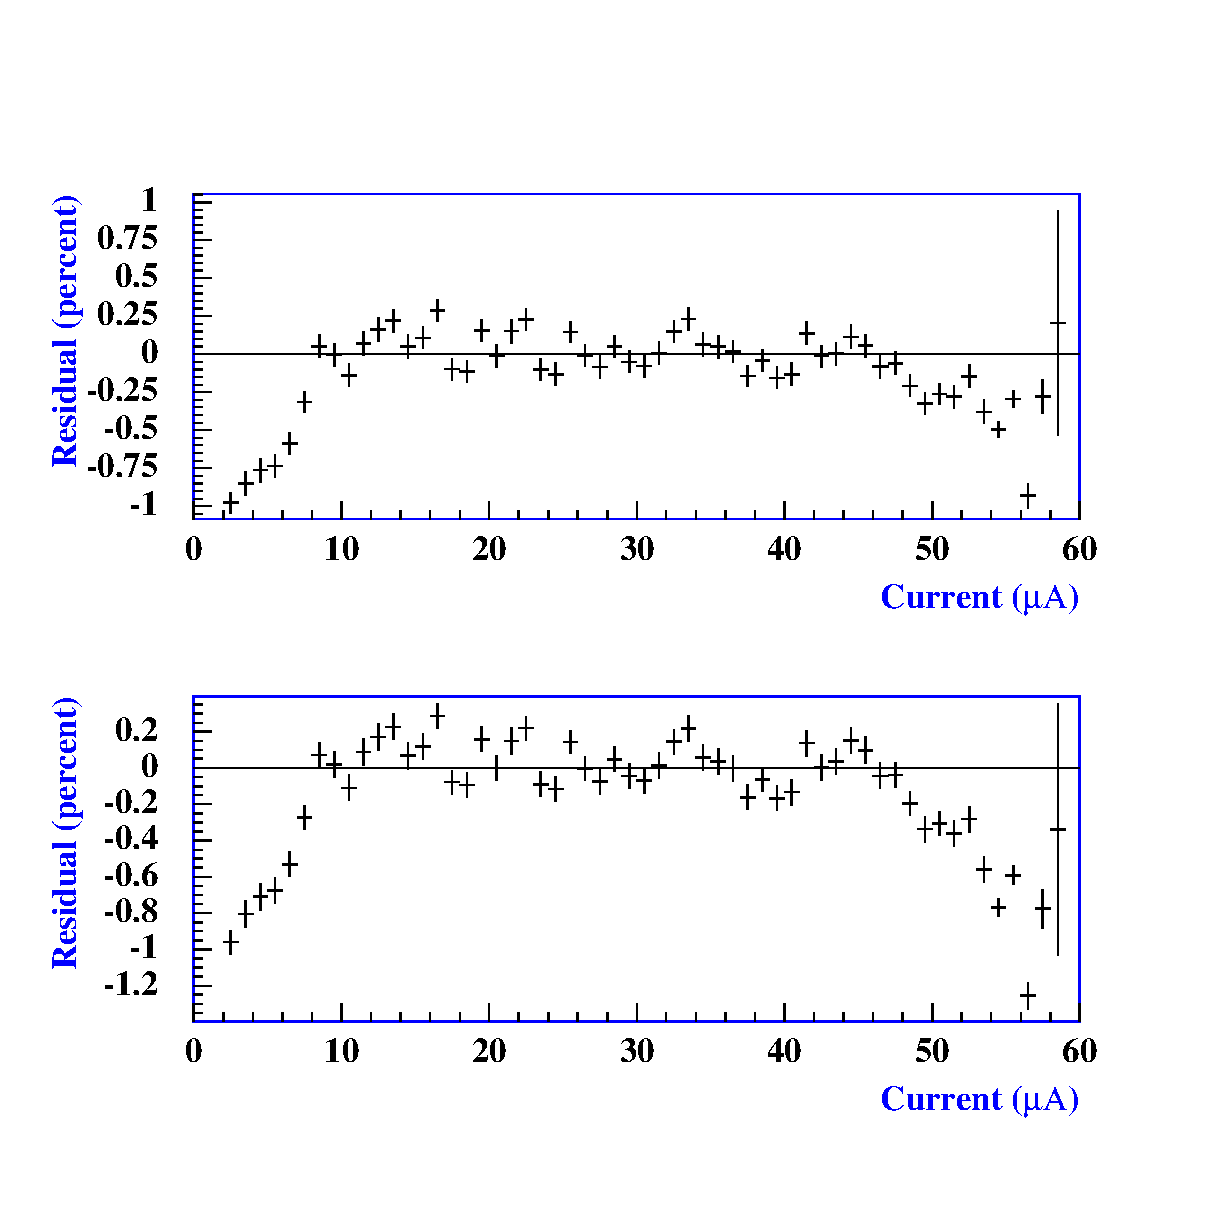
\includegraphics[width=3.5in]{DW/fig24_rsh_linearbu.eps}
\caption{(Color online) (top) Residuals from fit of BCM1 to Unser data, as a fraction
of the BCM1 pulse height at 32 $\mu$A, versus beam current.  (bottom)
Same for fit of BCM2 to Unser.}
% We need our own figure here.
\label{Fig24_RSH_Linearbu} 
\end{center}
\end{figure}

\begin{figure}
\begin{center}
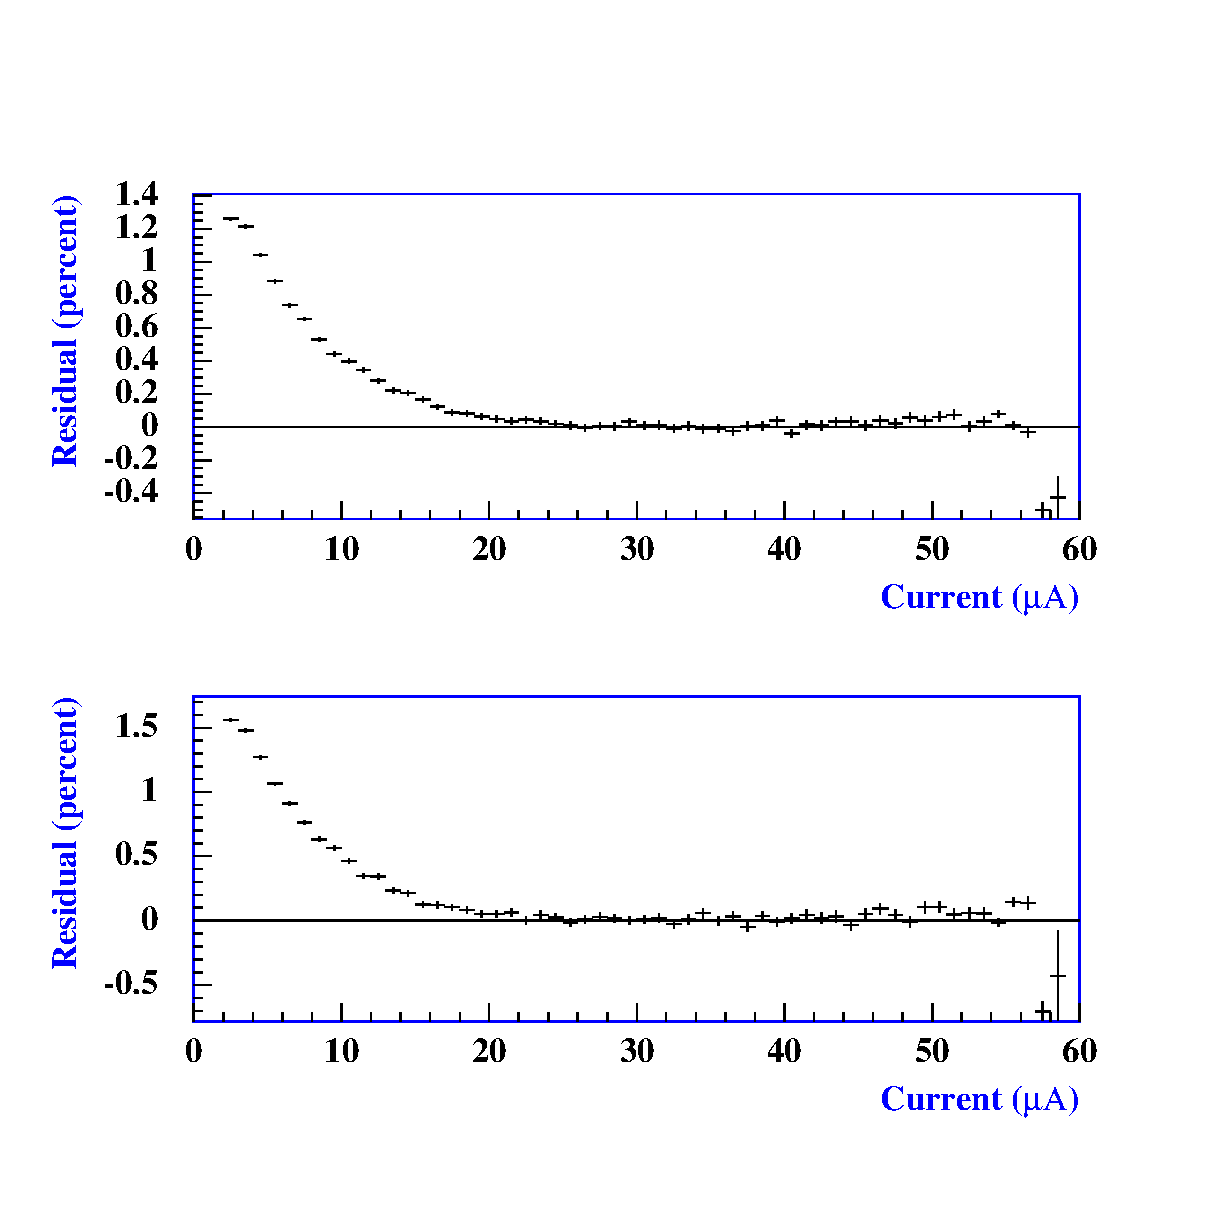
\includegraphics[width=3.5in]{DW/fig25_rsh_lineardb1.eps}
\caption{(Color online) (top) Residuals from fit of detector 1 to BCM1 data, as a fraction
of the detector 1 pulse height at 32 $\mu$A, versus beam current.  (bottom)
Same for fit of detector 2 to BCM1.}
% We need our own figure here.
\label{Fig25_RSH_Lineardb1} 
\end{center}
\end{figure}

Detector pedestals were measured by averaging the detector
signals during times when the beam is off.  The resulting pedestals
were always less than 0.3\% of the signal corresponding to the lowest
stable beam current in the production data set, and typically less
than 0.06\%; these pedestals are negligible.

The cavity monitor pedestals cannot be measured this way, since the
cavity signals are meaningless when the beam is off.  Instead, we fit
$I_{1(2)}$ to $I_U$ in the calibration data and extrapolate to zero
current.  Such an extrapolation requires knowledge of the average
Unser pedestal, which is obtained from the beam-off data in the same
run.  The resulting pedestals are less than 2\% of the signal
corresponding to the lowest stable beam current in the production data
set.

In conclusion, no corrections for pedestals or nonlinearities needed 
to be applied.  The nonlinearities of the detectors and cavity monitors
were negligible over the dynamic range of the beam current we ran.
The pedestals for detectors and cavity monitors were negligible.
